\section{Methodology}
\label{methodology}

The main goal of our research is to produce a complete, correct taxonomy of
software testing terminology. However, we cannot do this without understanding
its current state. Therefore, we start by documenting how the literature
currently uses testing terminology, both correctly and incorrectly. This
results in a big messy glossary of software testing terms, along with a list of
flaws. Once we analyze these data, including how and why these flaws emerge, we
can start to resolve them. For now, we document the current (messy) state of
software testing terminology by:

\input{build/methodOverview}

\subsection{Sources}\label{sources}
As there is no single authoritative source on software testing terminology,
we need to look at many sources to observe how this terminology is used in
practice. Since we are particularly interested in software engineering, we
start from the vocabulary document for systems and software engineering%
\qtodo{Better name for this?}
\citep{IEEE2017} and two versions of the \acf{swebok}---the newest
one \citep{SWEBOK2014} and one submitted for public review\footnote{
    \refHelper \citep{SWEBOK2024} has been published since we investigated
    these sources; if time permits, we will revisit this published version.
} \citep{SWEBOK2024}. To gather further sources, we then use a version of
``snowball sampling'',
which ``is commonly used to locate hidden populations \dots{} [via] referrals
from initially sampled respondents to other persons'' \citep{Johnson2014}. We
apply this concept to ``referrals'' between sources. \addTextEx{} We similarly
``snowball'' on terminology itself; when a term requires more investigation
(e.g., its definition is missing or unclear), we perform a
miniature literature review on this subset to ``fill in'' this missing
information (see \Cref{undef-terms}). We may then investigate these additional
sources in their entirety, as opposed to just the original subset of interest,
based on their trustworthiness (defined in \Cref{trust}) and how much extra
information they provide.

For ease of discussion and analysis, we group the complete set of sources into
``tiers'' based on their format, method of publication, and our heuristic of
trustworthiness (defined in \Cref{trust}). We therefore create the
following tiers, given in order of descending trustworthiness:
\begin{enumerate}
    \item established standards (\Cref{stds}),
    \item terminology collections (\Cref{metas}),
    \item textbooks (\Cref{texts}), and
    \item papers and other documents (\Cref{papers}).
\end{enumerate}
A summary of how many sources comprise each tier is given in
\Cref{fig:sourceSummary}\ifnotpaper; complete lists of sources for each tier
are given in \Cref{app-src-tiers}\fi. We often use papers to ``fill in'' missing
information in a more specific subdomain and do not always investigate them
entirely (see \Cref{undef-terms}), which results in a large number of them. We
use standards the second most frequently due to their high trustworthiness and
broad scope; for example, the glossary portion of \citep{IEEE2017} has 514
pages! Using these standards allows us to record many test approaches in a
similar context from a source that is widely used and well-respected.

% Only top or bottom to comply with IEEE guidelines
\begin{figure}[bt!]
    \centering
    \begin{tikzpicture}
        \pie[sum=auto, after number=, text=legend, thick,
            scale=\ifnotpaper0.7\else0.5\fi,
            every label/.style={align=left, scale=0.7}]
        {\stdSources{3}/\stds{},
            \metaSources{3}/\metas{},
            \textSources{3}/\texts{},
            \paperSources{3}/\papers{}}
    \end{tikzpicture}
    \caption{Summary of how many sources comprise each source tier.}
    \label{fig:sourceSummary}
\end{figure}

\subsubsection{\stdSources{1}}
\label{stds}
% Colored \textcolor{green}{green}

These are documents written for the field of software engineering by reputable
standards bodies, namely ISO, the \acf{iec}, and IEEE. Their purpose is to
``encourage the use of systems and software engineering standards'' and
``collect and standardize terminology'' by ``provid[ing] definitions that are
rigorous, uncomplicated, and understandable by all concerned''
\citep[p.~viii]{IEEE2017}. For these reasons, they
are the most trustworthy sources. However, this does not imply perfection, as we
identify \stdFlawDmnBrkdwn{13} % is (should be!) equal to \stdFlawMnfstBrkdwn{13}
flaws within these standards (see \Cref{tab:flawMnfsts,tab:flawDmns})!
Only standards for software development and testing are in scope for
this research (see \Cref{scope}). For example, ``the purpose of the
ISO/IEC/IEEE 29119 series is to define an internationally agreed set of
standards for software testing that can be used by any organization when
performing any form of software testing''
\ifnotpaper(\fi\citeyear[p.~vii]{IEEE2022}\ifnotpaper; similar in
\citeyear[p.~ix]{IEEE2016})\fi.

\subsubsection{\metaSources{1}}
\label{metas}
% Colored \textcolor{blue}{blue}

These are collections of software testing terminology built up from multiple
sources, such as the established standards outlined in \Cref{stds}. For
example, the \acs{swebok} is ``proposed as a
suitable foundation for government licensing, for the regulation of software
engineers, and for the development of university curricula in software
engineering'' \citep[p.~xix]{KanerEtAl2011}. Even though it is ``published by
the IEEE Computer Society'', it ``reflects the current state of generally
accepted, consensus-driven knowledge derived from the interaction between
software engineering theory and practice'' \citep{AboutSWEBOK}. Due to this
combination of IEEE standards and state-of-the-practice observations, we
designate it as a collection of terminology as opposed to an established
standard. Collections such as this are often written by a large
organization, such as the \acf{istqb}, but not always. \ifnotpaper \else
    \citeauthor{Firesmith2015} \fi \citet{Firesmith2015}'s taxonomy presents
relations between many test approaches and \ifnotpaper \else
    \citeauthor{DoğanEtAl2014} \fi \citet{DoğanEtAl2014}'s literature
review cites many sources from which we can ``snowball'' if desired
(see \Cref{sources}), so we include them in this tier as well.

\subsubsection{\textSources{1}}
\label{texts}
% Colored \textcolor{Maroon}{maroon}

We consider textbooks to be more trustworthy than papers (see \Cref{papers})
because they are widely used as resources for teaching software engineering and
industry frequently uses them as guides. Although textbooks have smaller sets of
authors, they follow a formal review process before publication. Textbooks used
at McMaster University \citep{Patton2006,PetersAndPedrycz2000,vanVliet2000}
served as the original (albeit ad hoc and arbitrary) starting point of this
research, and we investigate other books as they arise. \addTextEx{}

\subsubsection{\paperSources{1}}
\label{papers}
% Colored black

The remaining documents all have much smaller sets of authors and are much less
widespread than those in higher source tiers. While most of these are journal
articles and conference papers, we also include the following document types.
Some of these are not peer-reviewed works but are still useful for
observing how terms are used in practice\thesisissueref{89}:

\begin{itemize}
    \item Report \citep{Kam2008,Gerrard2000a,Gerrard2000b}
    \item Thesis \citep{Bas2024}
          % \item A less-formal classification \citep{KuļešovsEtAl2013}
    \item Website \citep{LambdaTest2024,Pandey2023}
    \item Booklet \citep{SPICE2022}
    \item \ifnotpaper \else ChatGPT \fi \citet{ChatGPT2024} (with its claims
          supported by \citet{RusEtAl2008})
\end{itemize}

% Moved here to display nicely in paper
\ifnotpaper\else
    % Only top or bottom to comply with IEEE guidelines
    \begin{table*}[t!]
        \ieeeCatsTable{}
    \end{table*}
\fi

\subsection{Procedure}
\label{procedure}

We track terminology used in the literature by building glossaries. The one
most central to our research is \ourApproachGlossary{}, where we give each
test approach its own row to record its name and any given \approachFields{}.
If no category is given, the ``approach'' category is assigned
(with no accompanying citation) as a ``catch-all'' category. All other fields
may be left blank, but a lack of definition indicates that the approach should
be investigated further to see if its inclusion is meaningful (see
\Cref{undef-terms}). Any additional information from other sources is added to
or merged with the existing information in our glossary where appropriate.
This includes the generic ``approach'' category being replaced with a more
specific one, an additional synonym being mentioned, or another source
describing an already-documented parent-child relation. If any new information
contradicts existing information (or otherwise indicates something is wrong),
this is investigated and documented (see \Cref{flaws}), which may be done
in a separate document and/or in the glossary itself. Sometimes, new
information does not conflict with existing information, in which case the
clearest and most concise version is kept, or they are merged to paint a more
complete picture. Finally, we record any other notes, such as questions,
prerequisites, and other resources to investigate.

We use similar procedures to track software qualities \ifnotpaper (see
    \Cref{qual-test}) \fi and supplementary terminology (either shared by
multiple approaches or too complicated to explain inline) in separate
glossaries with a similar format. This includes recording the name, definition,
and synonym(s) of these terms, as well as any precedence for a related test
type for a given software quality. For example, analyzability\footnote{
    This may be spelled ``analyzability'' \citep[p.~18]{IEEE2017} or
    ``analysability'' \citep{ISO_IEC2023a}; since this is a dialectal
    difference, we do not count this as a label flaw (see
    \Cref{label-flaw-def}).}, modifiability, modularity, reusability, and
testability are all subqualities of maintainability \ifnotpaper
    (\citealp{ISO_IEC2023a}; \citealp[Tab.~A.1]{IEEE2021};
    \citealp[p.~7\=/10]{SWEBOK2024}) \else
    \cite[p.~7\=/10]{SWEBOK2024}, \cite[Tab.~A.1]{IEEE2021},
    \cite{ISO_IEC2023a} \fi which has an associated test type
\ifnotpaper
    (\citealp[pp.~5, 22]{IEEE2022}; \citeyear[p.~38, Tab.~A.1]{IEEE2021})\else
    \cite[pp.~5, 22]{IEEE2022}, \cite[p.~38, Tab.~A.1]{IEEE2021}\fi. This sets
a ``precedent'' for each of these subqualities having its own associated test
type (e.g., reusability testing).

We use heuristics to guide this process for all three
glossaries to increase confidence that all terms are identified, paying
special attention to the following when investigating a new source:
\begin{itemize}
    \item glossaries and lists of terms,
    \item testing-related terms (e.g., terms containing ``test(ing)'',
          \ifnotpaper ``review(s)'', ``audit(s)'', \fi
          ``validation'', or ``verification''),
    \item terms that had emerged as part of already-discovered
          testing approaches, \emph{especially} those that were ambiguous
          or prompted further discussion (e.g., terms containing
          ``performance'', ``recovery'', ``component'', ``bottom-up'',
          \ifnotpaper ``boundary'', \fi or ``configuration''), and
    \item terms that implied testing approaches%
          \ifnotpaper\footnote{
                  Since these methods for deriving test approaches only arose
                  as research progressed, some examples would have been missed
                  during the first pass(es) of resources investigated earlier
                  in the process. While reiterating over them would be ideal,
                  this may not be possible due to time constraints.
              } (see \Cref{derived-tests})\fi.
\end{itemize}
We apply these heuristics to most investigated sources, especially established
standards (see \Cref{stds}), in their entirety. Some sources, however, are only
partially investigated, such as those chosen for a specific area of
interest or based on a test approach that was determined to be out-of-scope.
These include the following sources as described in \Cref{undef-terms}:
\citep{ISO2022,ISO2015,Dominguez-PumarEtAl2020,PierreEtAl2017,
    TrudnowskiEtAl2017,YuEtAl2011,Tsui2007,Goralski1999}.

During the first pass of data collection, we investigate and record all
terminology related to software testing. Some of these terms are less
applicable to test case automation---our original motivation---%
\ifnotpaper(such as static testing; see \Cref{static-test}%
\thesisissueref{39})\ \fi%
or quite broad\ifnotpaper\ (such as attacks; see \Cref{attacks}%
    \thesisissueref{55})\fi, so they will be omitted during future analysis.
\ifnotpaper
    Others are so vague that they do not provide any new, meaningful
    information. For example, the ``systematic determination of the extent to
    which an entity meets its specified criteria'' \citep[p.~167]{IEEE2017} is
    certainly relevant to testing software; while this definition of
    ``evaluation'' may be meaningful when defining software testing generally,
    it does not define a new approach or procedure and applies much more
    broadly than just to testing. We decided\thesisissueref{39,44,28} that the
    following terms are too vague to merit tracking in our glossaries or
    analyzing further:
    \begin{itemize}
        \item \textbf{Evaluation:} the ``systematic determination of the extent
              to which an entity meets its specified criteria''
              \citep[p.~167]{IEEE2017}
        \item \textbf{Product Analysis:} the ``process of evaluating a product by
              manual or automated means to determine if the product has certain
              characteristics'' \citep[p.~343]{IEEE2017}
        \item \textbf{Quality Audit:} ``a structured, independent process to
              determine if project activities comply with organizational and
              project policies, processes, and procedures'' \citep[p.~361]{IEEE2017}
              \todo{OG PMBOK}
        \item \textbf{Software Product Evaluation:} a ``technical operation that
              consists of producing an assessment of one or more characteristics
              of a software product according to a specified procedure''
              \citep[p.~424]{IEEE2017}
    \end{itemize}

    \phantomsection{}\label{infers}
    Throughout this process, information can be inferred from ``surface-level''
    analysis that follows straightforwardly but isn't explicitly stated by any
    source. Examples of this are large scale integration testing and legacy
    system integration testing, described by \citeauthor{Gerrard2000a} in
    \citeyearpar[p.~30]{Gerrard2000b} and (\citeyear[Tab.~2]{Gerrard2000a};
    \citeyear[Tab.~1]{Gerrard2000b}), respectively. While he never explicitly
    says so, it can be inferred that these approaches are children of
    integration testing and system integration testing, respectively.
    Although these data do not come from the literature, they are documented
    for completeness; inferred flaws are given in \Cref{infer-flaws}
    and inferred relations, if any, are included in \recFigs{}.
\fi

\subsubsection{Derived Test Approaches}
\label{derived-tests}

Throughout this research, we noticed many groups of test approaches that arise
from some underlying area of software (testing) knowledge. The legitimacy of
extrapolating new test approaches from these knowledge domains is heavily
implied by the literature, but not explicitly stated as a general rule. Regardless,
since the field of software is ever-evolving, it is crucial to be able to
adapt to, talk about, and understand new developments in software testing.
Bases for defining new test approaches suggested by the literature include
coverage metrics, software qualities, and attacks. These are meaningful
enough to merit analysis and are therefore in scope. Requirements may also
imply related test approaches, but this mainly results in test approaches
that would be out of scope. Other test approaches found in the literature
are derived from programming languages or other orthogonal test approaches,
but these are out of scope as this information is better captured by other
approaches.

\ifnotpaper
    \paragraph{Coverage-driven Techniques}
    \label{cov-test}

    Test techniques are able to ``identify test coverage items \dots{} and
    derive corresponding test cases''
    \ifnotpaper
        (\citealp[p.~11]{IEEE2022}; similar in \citeyear[p.~467]{IEEE2017})
    \else
        \cite[p.~11]{IEEE2022} (similar in \cite[p.~467]{IEEE2017})
    \fi
    in a ``systematic'' way
    \citeyearpar[p.~464]{IEEE2017}.
    \ifnotpaper
        This allows for ``the coverage achieved by a specific test design
        technique'' to be calculated as a percentage of ``the number of test
        coverage items covered by executed test cases'' \citeyearpar[p.~30]{IEEE2021}.
        %     ``Coverage levels can range
        %     from 0\% to 100\%'' and may or may not include ``infeasible'' test coverage
        %     items, which are ``not \dots{} executable or [are] impossible to be covered by a
        %     test case'' \citetext{p.~30}. Perhaps more interestingly, the further
        %     implication is
        % \else
        %     This means
    \fi % that
    Therefore, a given coverage metric implies a test approach aimed to
    maximize it. For example, path testing ``aims to execute all entry-to-exit
    control flow paths in a \acs{sut}'s control flow graph'' \citep[p.~5-13]{SWEBOK2024},
    thus maximizing the path coverage
    \ifnotpaper
        \citep[see][Fig.~1\thesisissueref{63}]{SharmaEtAl2021}\else
        (see \cite[Fig.~1]{SharmaEtAl2021}\thesisissueref{63})\fi.

    \paragraph{Quality-driven Types}
    \label{qual-test}

    Since test types are ``focused on specific quality characteristics''
    \ifnotpaper
        (\citealp[p.~15]{IEEE2022}; \citeyear[p.~7]{IEEE2021};
        \citeyear[p.~473]{IEEE2017}\todo{OG IEEE 2013})%
    \else
        \cite[p.~15]{IEEE2022}, \cite[p.~7]{IEEE2021}, \cite[p.~473]{IEEE2017}%
    \fi, they can be derived from software qualities: ``capabilit[ies] of
    software product[s] to satisfy stated and implied needs when used under
    specified conditions'' \citep[p.~424]{IEEE2017}\todo{OG ISO/IEC 2014}. This
    is supported by reliability and performance testing, which are both examples of
    test types \citep{IEEE2022, IEEE2021} that are based on their underlying
    qualities \citep[p.~18]{FentonAndPfleeger1997}.
    % \ifnotpaper
    %     For quantifying quality-driven testing, measurements should include
    %     an entity to be measured, a specific attribute to measure, and the actual
    %     measure (i.e., units, starting state, ending state, what to include)
    %     \citetext{p.~36} where attributes must be
    %     defined before they can be measured \citetext{p.~38}.
    %
    % \fi
    Given the importance of software qualities to defining test types, the
    definitions of \qualityCount{} software qualities are also tracked in this
    current work\thesisissueref{21,23,27}. This was done by capturing their
    definitions, any precedent for the existence of an associated test type,
    and any synonyms (see \Cref{syn-rels}) and additional notes in a glossary.
    Software qualities are ``upgraded'' to test types when mentioned (or
    implied) by a source by adding an associated test approach to this glossary
    (as outlined in \Cref{procedure}) and removing the quality entry. Examples
    of this include conformance testing \ifnotpaper
        (\citealp[p.~5\=/7]{SWEBOK2024}; \citealp[p.~25]{JardEtAl1999}; implied
        by \citealp[p.~93]{IEEE2017})\else \cite[p.~5\=/7]{SWEBOK2024},
        \cite[p.~25]{JardEtAl1999}\fi, efficiency testing
    \citep[p.~44]{Kam2008}, and survivability testing \citep[p.~40]{GhoshAndVoas1999}.

    \paragraph{Attacks}
    \label{attacks}
    While attacks can be ``malicious'' \citep[p.~7]{IEEE2017}, they are also
    given as a test practice (\citeyear[p.~34]{IEEE2022}; see \Cref{tab:multiCats}).
    This means that software attacks, such as code injection and password
    cracking \citepISTQB{}, can also be used for testing software, and only
    this kind of software attack is in scope. This is supported by the fact
    that penetration testing is also called ``ethical hacking testing''
    \citep[p.~13-4]{SWEBOK2024} or just ``ethical hacking''
    \citep[p.~28]{Gerrard2000b}; while hacking in general is not a test
    approach, doing so systematically to test and improve the software is.

    \paragraph{Requirements-driven Approaches}
    \label{req-test}
    While not as universally applicable, some types of requirements have associated
    types of testing (e.g., functional, non-functional, security). This may mean
    that categories of requirements \emph{also} imply related testing approaches
    (such as ``technical testing''). \ifnotpaper Even assuming this is the case, some types of
        requirements do not apply to the code itself, and as such are out of scope%
        \thesisissueref{43}, such as:
        \begin{itemize}
            \item \textbf{Nontechnical Requirement:} a ``requirement affecting product
                  and service acquisition or development that is not a property of
                  the product or service'' \citep[p.~293]{IEEE2017}
            \item \textbf{Physical Requirement:} a ``requirement that specifies a
                  physical characteristic that a system or system component must
                  possess'' \citep[p.~322]{IEEE2017}
        \end{itemize}
    \fi

    \paragraph{Language-specific Approaches}
    \label{lang-test}
    Specific programming languages are sometimes used to define test approaches.
    If the reliance on a specific programming language is intentional, then
    this really implies an underlying test approach that may be generalized to
    other languages. These are therefore considered out-of-scope\thesisissueref{63},
    including the following examples:

    \begin{itemize}
        \item ``An approach \dots{} for JavaScript testing
              (referred to as Randomized)'' \citep[p.~192]{DoğanEtAl2014} is
              really just random testing used within JavaScript.
        \item ``SQL statement coverage'' is really just statement coverage
              used specifically for SQL statements \citep[Tab.~13]{DoğanEtAl2014}%
              \todo{OG Alalfi et al., 2010}.
        \item Testing for ``faults specific to PHP'' is just a subcategory of
              fault-based testing, since ``execution failures \dots{} caused by
              missing an included file, wrong MySQL quer[ies] and uncaught
              exceptions'' are not exclusive to PHP
              \citep[Tab.~27]{DoğanEtAl2014}\todo{OG Artzi et al., 2008}.
        \item While ``HTML testing'' is listed or implied by
              \citeauthor{Gerrard2000a} (\citeyear[Tab.~2]{Gerrard2000a};
              \citeyear[Tab.~1, p.~3]{Gerrard2000b}) and
              \citet[p.~220]{Patton2006}, it seems to be a combination of syntax
              testing, functionality testing, hyperlink testing/link checking,
              cross-browser compatibility testing, performance testing,
              content checking \citep[p.~3]{Gerrard2000b}, and grey-box testing
              \citep[pp.~218\==220]{Patton2006}.
    \end{itemize}

    \paragraph{Orthogonally Derived Approaches}
    \label{orth-test}
    Some test approaches appear to be combinations of other (seemingly
    orthogonal) approaches. While the use of a combination term can sometimes
    make sense, such as when writing a paper or performing testing that focuses
    on the intersection between two test approaches, they are sometimes given
    the same ``weight'' as their atomic counterparts. For example, \citetISTQB{}
    \multiAuthHelper{include} ``formal reviews'' and ``informal reviews'' in
    \ifnotpaper their \else its \fi glossary as separate terms, despite their
    definitions essentially boiling down to ``reviews that follow (or do not
    follow) a formal process'', which do not provide any new information.
    We consider these out of scope if their details are captured by their
    in-scope subapproaches, but record them as support for the orthogonality of
    test approach categories in \Cref{orth-test-exs}. If a source describes an
    orthogonally derived approach in more detail, such as security audits, we
    also record it as a distinct approach in \ourApproachGlossary{} with its
    related information.

    The existence of orthogonal combinations could allow for other test
    approaches to be extrapolated from them. For example, \citet{Moghadam2019}
    uses the phrase ``machine learning-assisted performance testing''; since
    performance testing is a known test approach, this may imply the existence
    of the test approach ``machine learning-assisted testing''. Likewise,
    \citet{JardEtAl1999} \multiAuthHelper{use} the phrases ``local synchronous
    testing'' and ``remote asynchronous testing''. While these can be
    decomposed, for example, into local testing and synchronous testing,
    the two resulting approaches may not be orthogonal, potentially even having
    a parent-child relation (defined in \Cref{par-chd-rels}).
\fi

\subsubsection{Undefined Terms}
\label{undef-terms}

The literature mentions many software testing terms without defining them.
While this includes test approaches, software qualities, and more general
software terms, we focus on the former as the main focus of our research.
In particular, many undefined test approaches are given by \ifnotpaper
    \citep{IEEE2022} and \citep{Firesmith2015}\else
    \cite{Firesmith2015} and \cite{IEEE2022}\fi. Once we exhaust the standards
in \Cref{stds}, we
perform miniature literature reviews on these subsets to ``fill in'' the
missing definitions (along with any relations), essentially ``snowballing''
on these terms. This process uncovers even more approaches, although some are
out of scope, such as \acf{emsec} testing\ifnotpaper, \else\ and \fi
aspects of \acf{orthat} \ifnotpaper and loop testing (see \Cref{hard-test}),
    and HTML testing (see \Cref{lang-test})\else (see \Cref{scope})\fi. The
following terms (and their respective related terms) were explored in the
sources given:
\input{build/undefTerms}
Applying our procedure from \Cref{procedure} to these sources brings the number
of testing approaches from \the\TotalBefore{} to \the\TotalAfter{} and the
number of \emph{undefined} terms from \the\UndefBefore{} to \the\UndefAfter{}%
\ifnotpaper\ (see \Cref{fig:undefPies})\fi. This implies that about
\the\numexpr 100 - 100 * (\UndefAfter - \UndefBefore) / (\TotalAfter -
\TotalBefore)\relax\% of added test approaches are defined, which helps verify
that our procedure constructively uncovers new terminology.

\ifnotpaper
    \begin{figure*}[hbtp!]
    \begin{subfigure}[c]{0.35\linewidth}
        \centering
        \begin{tikzpicture}[thick, scale=0.7, every label/.style={align=left, scale=0.7}]
            \pie[text=inside, sum=auto, color={blue!60, orange!60}]{
                {\the\numexpr \TotalBefore - \UndefBefore\relax}/,
                {\the\UndefBefore}/
            }
        \end{tikzpicture}
        \caption{The \the\TotalBefore{} approaches before investigating undefined terms.}
        \label{fig:undefPiesBefore}
    \end{subfigure}
    \hfill
    \begin{subfigure}[c]{0.35\linewidth}
        \centering
        \begin{tikzpicture}[thick, scale=0.7, every label/.style={align=left, scale=0.7}]
            \pie[text=inside, sum=auto, color={blue!60, orange!60}]{
                {\the\numexpr \TotalAfter - \UndefAfter\relax}/,
                {\the\UndefAfter}/
            }
        \end{tikzpicture}
        \caption{The \the\TotalAfter{} approaches after investigating undefined terms.}
        \label{fig:undefPiesAfter}
    \end{subfigure}
    \hfill
    \begin{subfigure}[c]{0.2\linewidth}
        \centering
        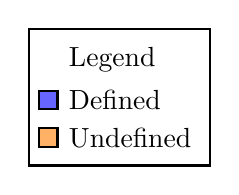
\begin{tikzpicture}
            \matrix [thick, draw=black] {
            \node[label=right:{Legend}] {}; \\
            \node[thick, shape=rectangle, draw=black, fill=blue!60,   label=right:{Defined}](0) {}; \\
            \node[thick, shape=rectangle, draw=black, fill=orange!60, label=right:{Undefined}](1) {}; \\
            };
        \end{tikzpicture}
    \end{subfigure}
    \caption{Breakdown of how many test approaches are undefined.}
    \label{fig:undefPies}
\end{figure*}

\fi

\phantomsection{}\label{missingTerms}
In addition to terms with missing definitions, some terms do not appear in
the literature at all! While most test approaches arise as a result of our
snowballing approach, we each have preexisting knowledge of what test
approaches exist (a form of experience-based testing, if you will).
As an example, we are surprised that property-based testing is not mentioned
in any sources investigated, even using it as a target ``stopping point''
throughout this process\thesisissueref{57,81,88,125}\qtodo{I think these issue
    refs, along with some others may actually be worth keeping in our final
    thesis/paper; thoughts?}. Test approaches such as these that arise
independently of snowballing may serve as starting points for continuing
research if they are not mentioned by the literature. The following terms come
from previous knowledge, conversations with colleagues, research for other
projects, or ad hoc cursory research to see what other test approaches exist:
\begin{minipage}{\linewidth}
    \begin{multicols}{2}
        \begin{enumerate}
            \item Chaos engineering
            \item Chosen-ciphertext \ifnotpaper\else \\ \fi attacks
            \item Concolic testing
            \item Concurrent testing
            \item Destructive testing
            \item Dogfooding
            \item Implementation-based testing
            \item \ifnotpaper Interaction-based \else \columnbreak
                      Interaction-based \\ \fi testing
            \item Lunchtime attacks\ifnotpaper%
                      \footnote{In previous meetings, Dr.~Smith mentioned
                          that with the number of test approaches that suggest
                          that people just like to label everything as
                          ``testing'', he would not be surprised if something
                          like ``Monday morning testing'' existed. While
                          independently researching chosen-ciphertext attacks
                          out of curiosity, this prediction of a time-based
                          test approach came true with ``lunchtime attacks''.}
                  \fi
            \item Parallel testing
            \item Property-based testing
            \item Pseudo-random bit \ifnotpaper\else \\ \fi testing
            \item Rubber duck testing
            \item Shadow testing
            \item Situational testing
        \end{enumerate}
    \end{multicols}
\end{minipage}
